\section{MTE-based Estimation of CM Effects}
\label{sec:controlfun}

The identification results suggest a direct three-step approach to estimating CM effects.
First, estimate the mediator propensity score using variation in treatment, the mediator instrument, and the remaining control variables.
Second, use the estimated propensity score to estimate the conditional-outcome function separately within each treatment arm.
Third, evaluate this function at the two treatment-induced mediator propensities.
Their difference estimates the AIE, while subtracting the estimated AIE from the ATE estimates the corresponding ADE.

For notational convenience, this section develops the estimator using the $Z_i=0$ subsample for the $m(\cdot;0,\vec X_i^-)$ estimation, which identifies $\operatorname{AIE}(0)$ and, consequently, $\operatorname{ADE}(1)$.
The corresponding estimators of $\operatorname{AIE}(1)$ and $\operatorname{ADE}(0)$ follow by applying the same procedure, starting with the $Z_i=1$ subsample.

\subsection{Semi-parametric MTE}
\label{sec:semiparametric-mte}

The first stage estimates the mediator propensity score,
\[
    \pi
    \big(
        z;
        \vec X_i^{\mathrm{IV}},
        \vec X_i^-
    \big)
    =
    \Probgiven{
        D_i=1
    }{
        Z_i=z,
        \vec X_i^{\mathrm{IV}},
        \vec X_i^-
    },
\]
and constructs the generated regressor
\( \widehat P_i
    =
    \widehat\pi
    \big(
        Z_i;
        \vec X_i^{\mathrm{IV}},
        \vec X_i^-
    \big) \).

The propensity score can be estimated using a correctly specified binary-response model or an appropriate semi-parametric estimator.
The identifying variation must come from $\vec X_i^{\mathrm{IV}}$, conditional on treatment and the remaining controls, and must generate the propensity-score support required by Assumption~\ref{mte:instrument}.

The second-stage now estimates the conditional-outcome function among the $Z_i=0$ subsample,
\[
    m
    \big(
        p;
        0,
        \vec x^-
    \big)
    =
    \Egiven{
        Y_i
    }{
        Z_i=0,
        P_i=p,
        \vec X_i^-=\vec x^-
    }.
\]
A convenient partially linear specification is
\[
    Y_i
    =
    \vec\phi_0'\vec X_i^-
    +
    s_0
    \big(
        \widehat P_i
    \big)
    +
    \varepsilon_{0,i},
    \qquad
    \text{for } i \in \{j \,: \, Z_j=0\},
\]
where $s_0(.)$ is approximated using a polynomial, regression spline, or another finite-dimensional sieve basis.
For a vector of known basis functions $\vec b_0(p)$, this can be written as
\[
    Y_i
    =
    \vec\phi_0'\vec X_i^-
    +
    \vec b_0
    \left(
        \widehat P_i
    \right)'
    \vec\rho_0
    +
    \epsilon_{0,i},
    \qquad
    \text{for } i:Z_i=0.
\]
The corresponding estimated conditional-outcome curve is constrcuted from the predictions, 
\(\widehat m
    \big(
        p;
        0,
        \vec x^-
    \big)
    =
    \widehat{\vec\phi}_0'\vec x^-
    +
    \vec b_0(p)'
    \widehat{\vec\rho}_0\).

The choice and dimension of $\vec b_0(p)$ must conform to the restricted-CF and rank conditions in Assumption~\ref{mte:restricted-cf}.
These conditions ensure that the finite IV-guided propensity-score support identifies the maintained approximation to the conditional-outcome curve over the mediator-complier interval.
\appendixref{appendix:mte-estimation} provides further details on the specification and estimation of this restricted outcome curve.\footnote{
    A parametric distributional assumption on the unobserved mediator-selection and outcome errors provides an alternative specification of $s_0(.)$.
    Joint normality, for example, produces the familiar inverse-Mills-ratio control function \citep{bjorklund1987estimation,heckman1979sample}.
    The semi-parametric approach used here instead approximates $s_0(.)$ with a polynomial, spline, or sieve basis and therefore does not require a parametric distribution for the unobserved errors.
}

Let
\( n_0 =
    \sum_{i=1}^{n} (1- Z_i) \)
denote the number of observations in the $Z_i=0$ subsample.
For each such observation, predict the $Z_i=0$ conditional outcome at the mediator propensities induced by both treatment states:
\[
    \widehat m
    \left(
        \widehat\pi
        \big(
            1;
            \vec X_i^{\mathrm{IV}},
            \vec X_i^-
        \big);
        0,
        \vec X_i^-
    \right), \text{ and }
    \widehat m
    \left(
        \widehat\pi
        \big(
            0;
            \vec X_i^{\mathrm{IV}},
            \vec X_i^-
        \big);
        0,
        \vec X_i^-
    \right).
\]
The difference between these predictions estimates the change in the $Z_i=0$ outcome surface caused by moving the mediator propensity from its value under $Z_i=0$ to its value under $Z_i=1$.
The sample-average estimator is
\[ \widehat{\operatorname{AIE}}(0)
    =
    \frac{1}{n_0}
    \sum_{i:Z_i=0}
    \Bigg[
        \widehat m
        \left(
            \widehat\pi
            \big(
                1;
                \vec X_i^{\mathrm{IV}},
                \vec X_i^-
            \big);
            0,
            \vec X_i^-
        \right)
        -
        \widehat m
        \left(
            \widehat\pi
            \big(
                0;
                \vec X_i^{\mathrm{IV}},
                \vec X_i^-
            \big);
            0,
            \vec X_i^-
        \right)
    \Bigg].
\]
Because $Z_i$ is quasi-randomly assigned, the covariate distribution in the $Z_i=0$ subsample consistently estimates the target population distribution.
The preceding sample average therefore consistently standardises the estimated conditional indirect effects to the target population.
A full-sample standardisation can alternatively be used as an efficiency refinement.

Evaluating the $Z_i=0$ outcome curve at the propensity score induced by $Z_i=1$ does not, by itself, constitute extrapolation.
The relevant requirement is that both evaluation points lie in the domain identified by mediator-instrument variation within the $Z_i=0$ arm.
When an endpoint is an observed propensity-score support point, the corresponding conditional mean is directly identified.
When an endpoint lies between supported values, its prediction is interpolation under the restricted-CF specification.
The mediator-complier support condition rules out evaluation outside the identified domain.

The complementary direct effect is estimated using the decomposition
\(
    \operatorname{ATE}
    =
    \operatorname{AIE}(0)
    +
    \operatorname{ADE}(1)
\).
Thus,
\(
    \widehat{\operatorname{ADE}}(1)
    =
    \widehat{\operatorname{ATE}}
    -
    \widehat{\operatorname{AIE}}(0),
\)
where $\widehat{\operatorname{ATE}}$ is estimated from the quasi-random assignment of $Z_i$, using a differences in means (conditional on $\vec X_i^-$) by any standard estimator.

This endpoint estimator avoids numerical differentiation.
The usual local-IV approach estimates the Mediator MTE from the derivative of a flexible conditional-outcome function with respect to the propensity score.
Derivatives of estimated nonparametric functions can be unstable, particularly near sparse regions of the support.
The present approach instead exploits the fact that the AIE is an integrated MTE: absolute continuity implies that its integral over the mediator-complier interval equals the difference between the conditional-outcome function evaluated at the two endpoints.
Estimation therefore requires only fitted values of $\widehat m(.)$, rather than an estimated derivative.

Standard series and sieve results establish consistency of the fitted conditional-outcome curve under the maintained smoothness, approximation, support, and basis-growth conditions.
Although the estimated function itself need not converge at a parametric rate, the sample-averaged endpoint difference is a smooth finite-dimensional functional and can be root-$n$ consistent and asymptotically normal under additional regularity conditions.
The effective sample size for estimating the $Z_i=0$ outcome curve is $n_0$; if $\frac{n_0}{n}$ converges to a positive constant, normalisation by $\sqrt{n_0}$ and $\sqrt n$ differs only by a constant scale factor.
\appendixref{appendix:semi-parametric} states the relevant consistency and asymptotic-normality conditions.

Inference must account for the generated propensity score, which enters both as a regressor in the outcome-curve estimation and as the argument at which the fitted curve is evaluated.
A practical approach is therefore to bootstrap the complete estimation procedure.
Each bootstrap iteration re-estimates the mediator propensity score, the restricted $Z_i=0$ outcome curve, both endpoint predictions, the AIE, and the ATE used to construct the ADE.

\subsection{Simulation Evidence}
\label{sec:simulations}
The following simulation gives an example to show how these methods work in practice.
Suppose data observed to the researcher $Z_i, D_i, Y_i, \vec X_i$ are drawn from the following data generating processes, for $i = 1, \hdots, N$, with 
$n = 5,000$ for this simulation.
\[ Z_i \sim \text{Binom}\left(0.5 \right),
    \;\; \vec X_i^- \sim N(4, 1),
    \;\; \vec X_i^{\text{IV}} \sim \text{Uniform}\left( -1, 1 \right), \]
\[ \left( U_i,(0,0), U_i(0,1), U_i(1,0), U_i(1,1), U_{C,i} \right) \sim
    N\left( \vec 0, \mat \Sigma \right) \]
$\mat \Sigma$ is the matrix of parameters which controls the level of confounding from unobserved costs and benefits.\footnote{
    The correlation and relative standard deviations for $U_i(.,0), U_i(.,1)$ affect how large selection bias in conventional CM estimates; correlation for these with unobserved costs $U_{C,i}$ does not particularly matter, though increased variance in unobserved costs makes estimates less precise for both OLS and MTE methods.
}

Each $i$ chooses to take mediator $D_i$ by a Roy model, with following mean definitions for each $z, d = 0, 1$
\begin{align*}
    D_i(z) &= \indicator{C_i \leq Y_i(z, 1) - Y_i(z, 0)},  \\
    \mu_{d}\left(z ; \vec X_i \right) &= \left( z + d + z d \right) + \vec X_i^-,
    \;\; \mu_{C}\left(z ; \vec X_i \right) = 3z + \vec X_i^- - \vec X_i^{\text{IV}}.
\end{align*}
Following \autoref{sec:regression}, these data have the following first and second-stage equations:
\begin{align*}
    D_i &= \indicator{U_{C,i} - \big( U_i(Z_i,1) - U_i(Z_i,0) \big)
    \leq 3z + \vec X_i^-  -\vec X_i^{\mathrm{IV}}},  \\
    Y_i &= Z_i + D_i + Z_i D_i + \vec X_i^- + \varepsilon_i.
\end{align*}
Treatment $Z_i$ has a causal effect on outcome $Y_i$, and it operates partially through mediator $D_i$.
Outcome mean $\mu_{D_i}\left( Z_i; \vec X_i \right)$ contains an interaction term, $Z_i D_i$, so while $Z_i,D_i$ have constant partial effects, the ATE depends on how many $i$ choose to take the mediator and there is causal effect heterogeneity.
$\varepsilon_i$ collects the normally distributed residuals, as in \autoref{sec:regression}.


After $Z_i$ is assigned, $i$ chooses to take mediator $D_i$ by considering the costs and benefits --- which vary based on $Z_i$, demographic controls $\vec X_i$, and the (non-degenerate) unobserved error terms $ \Big( U_i(z,d) \Big)_{z,d = 0,1}$.
As a result, sequential quasi-random assignment does not hold; the mediator is not conditionally ignorable.
Thus, a conventional approach to CM does not give an estimate for how much of the ATE goes through mediator $D$, but is contaminated by selection bias thanks to the unobserved error terms.

I simulate this data generating process 10,000 times, using
\[ \mat\Sigma =
    \begin{pmatrix}
        1 & 0.75 & 1 & 0.75 & 0 \\
        0.75 & 2.25 & 0.75 & 2.25 & 0 \\
        1 & 0.75 & 1 & 0.75 & 0 \\
        0.75 & 2.25 & 0.75 & 2.25 & 0 \\
        0 & 0 & 0 & 0 & 0.25
    \end{pmatrix}. \]
With these data simulated, I estimate CM effects with conventional CM methods (two-stage OLS) and the introduced MTE methods.\footnote{
    This choice of parameters has $U_i(0,d)$ following the same distribution as $U_i(1,d)$ (not differing across $Z_i =0,1$) for each $d=0,1$, and
    $\Var{U_i(., 0)} = 1, \Var{U_i(., 1)} = 2.25, \text{Corr}\big(U_i(., 0), U_i(., 1)\big) = 0.5$ so that unobserved errors meaningfully confound conventional CM methods, with notable heteroscedasticity.
    Unobserved costs are uncorrelated with $U_i(.,0), U_i(.,1)$ (although non-zero correlation would not meaningfully change the results), and $\Var{U_{C,i}} = 0.25$ maintains uncertainty in unobserved costs.
}
In this simulation $\Prob{D_i = 1} = 0.39$, and $45.8\%$ of the sample are mediator compliers (for whom $D_i(0)=0$ and $D_i(1)=1$).
This gives an ATE value of 2.13, AIE(0) 0.51 and ADE(1) 1.62, respectively.

\begin{figure}[!h]
    \caption{The MTE Approach Addresses Persistent Bias in Conventional CM Estimates.}
    \begin{subfigure}[c]{0.475\textwidth}
        \centering
        \caption{$\hat{\text{AIE}(0)} - \text{AIE}(0)$.}
        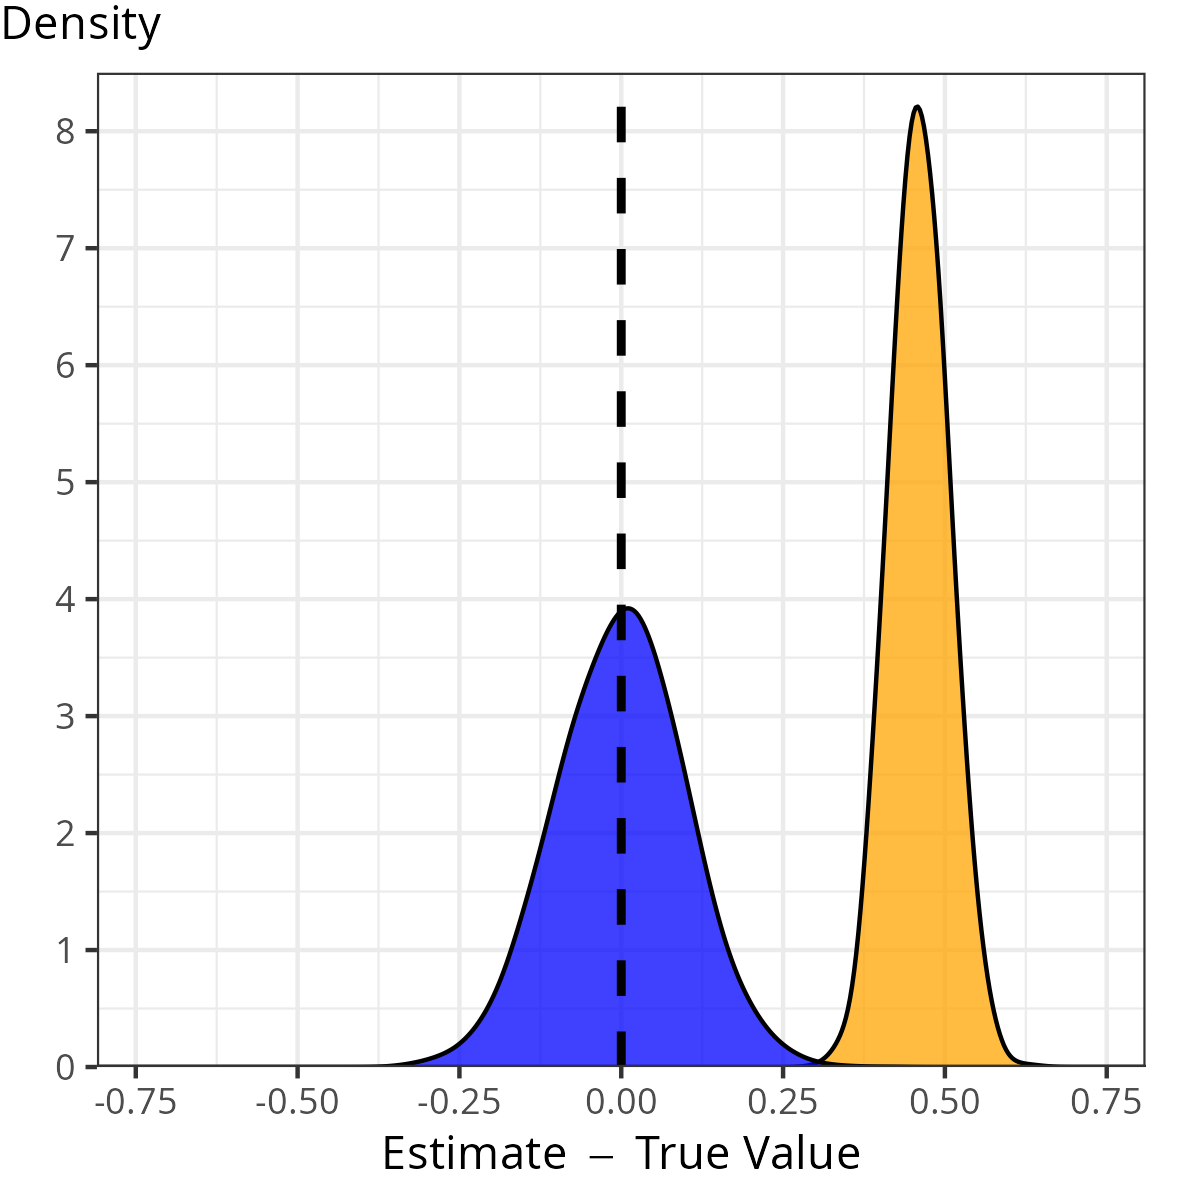
\includegraphics[width=\textwidth]{
            sections/figures/normal-indirect-dist.png}
    \end{subfigure}
    \begin{subfigure}[c]{0.475\textwidth}
        \centering
        \caption{$\hat{\text{ADE}(1)} - \text{ADE}(1)$.}
        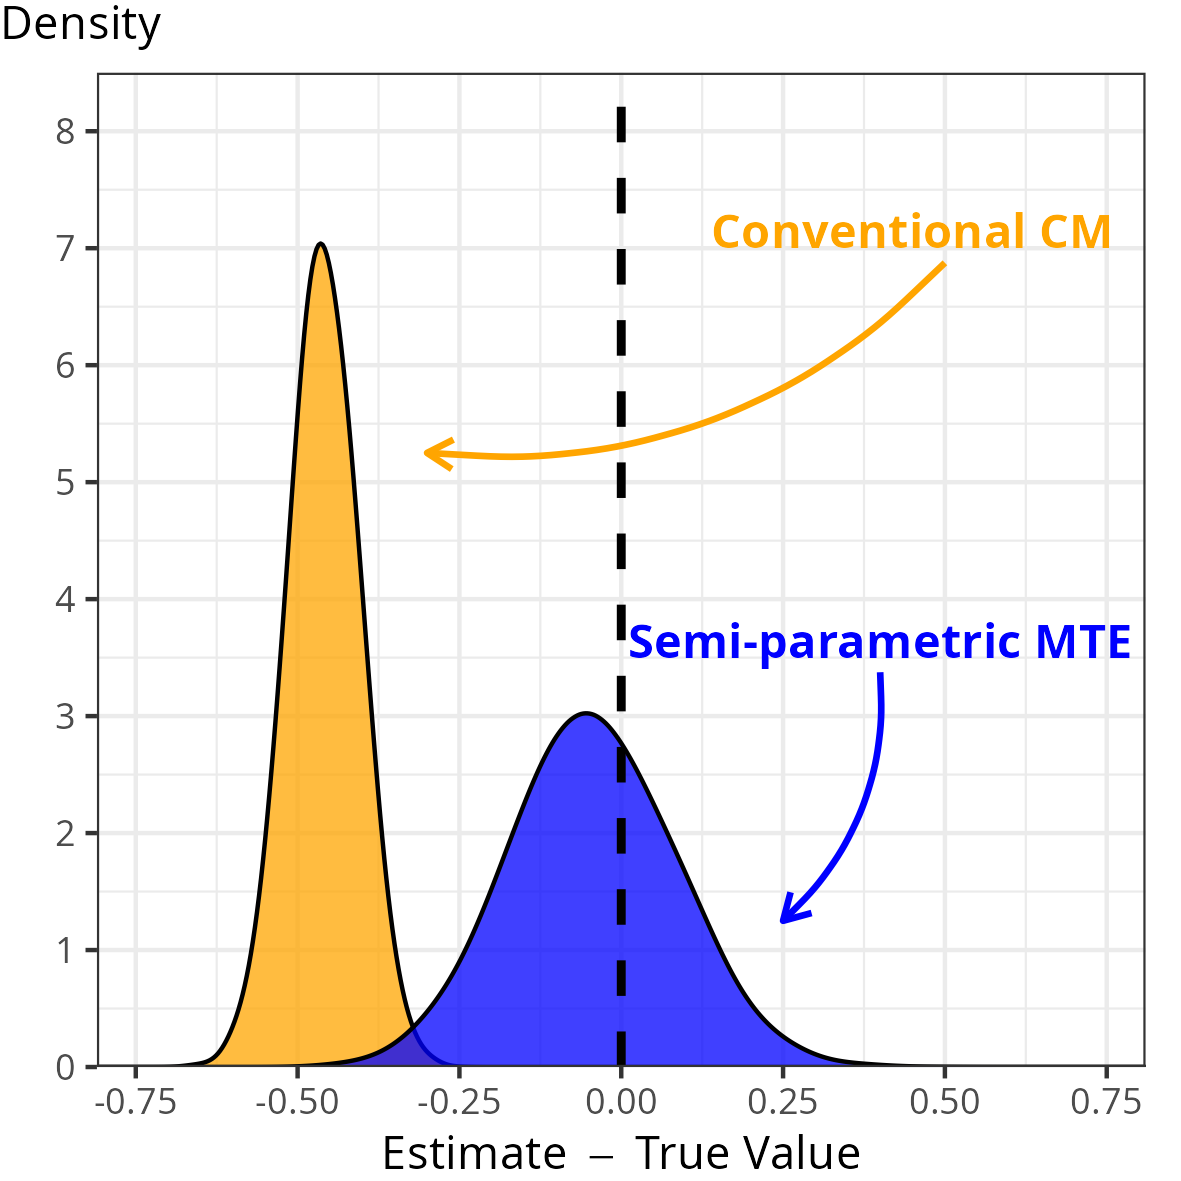
\includegraphics[width=\textwidth]{
            sections/figures/normal-direct-dist.png}
    \end{subfigure}
    \label{fig:cm-normal-dist}
    \justify
    \footnotesize
    \textbf{Note:}
    These figures show the empirical density of point estimates minus the true average effect, for 10,000 different datasets generated from a Roy model with normally distributed error terms (with both correlated error terms and heteroscedasticity, further described in \autoref{sec:simulations}).
    The black dashed line is the true value;
    orange is the distribution of conventional CM estimates from two-stage OLS \citep{imai2010identification},
    and blue estimates with a two-stage Heckman selection adjustment.
\end{figure}

\autoref{fig:cm-normal-dist} shows how these estimates perform, with a semi-parametric MTE approach, relative to the true value.
The OLS estimates' distribution do not overlap the true values for any standard level of significance; the distance between the OLS estimates and the true values are the underlying bias terms derived in \autoref{thm:selection-bias}.
The semi-parametric MTE approach perfectly reproduces the true values, as the probit first-stage correctly models the normally distributed error terms.

\begin{figure}[h!]
    \caption{MTE-Based Estimates Work with Different Error Term Parameters.}
    \begin{subfigure}[c]{0.475\textwidth}
        \centering
        \caption{AIE(0).}
        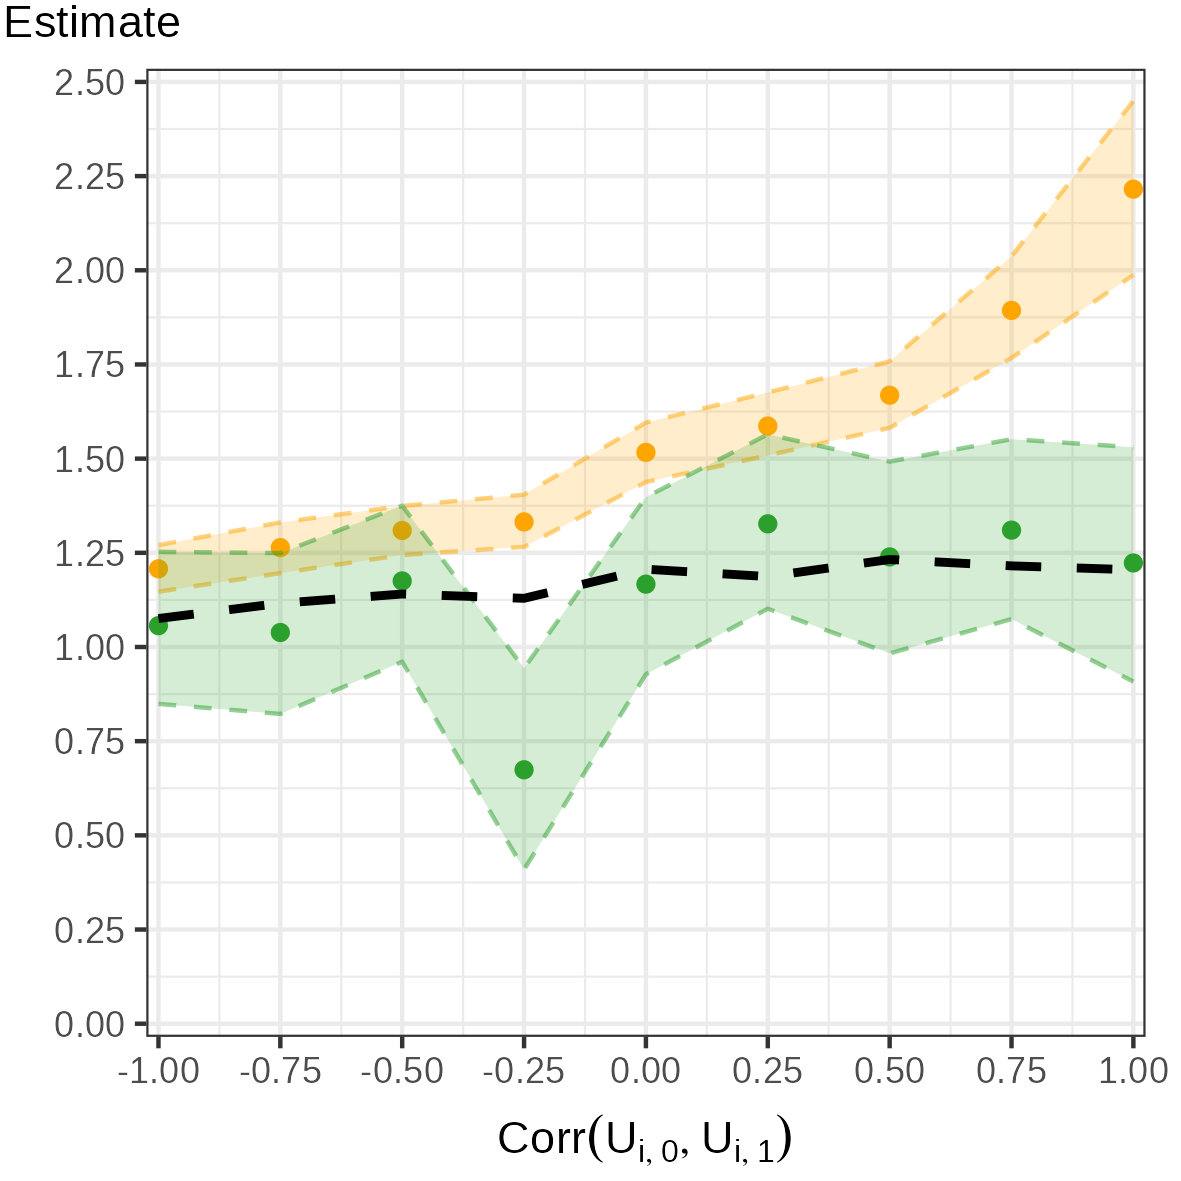
\includegraphics[width=\textwidth]{
            sections/figures/rho-indirecteffect-bias.png}
    \end{subfigure}
    \begin{subfigure}[c]{0.475\textwidth}
        \centering
        \caption{ADE(1).}
        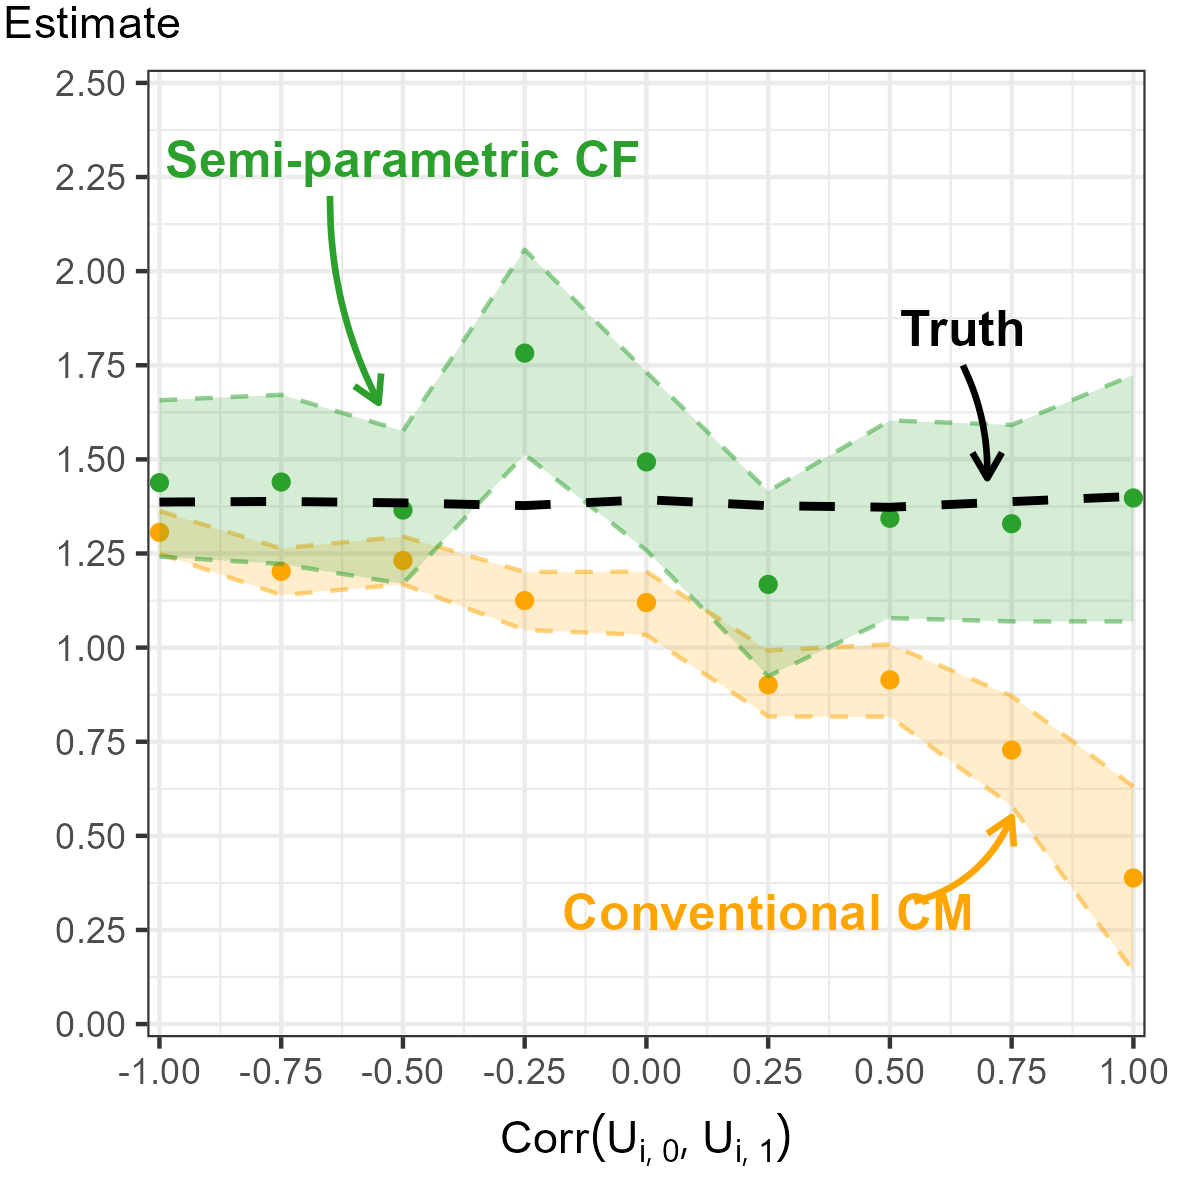
\includegraphics[width=\textwidth]{
            sections/figures/rho-directeffect-bias.png}
    \end{subfigure}
    \label{fig:rho-bias}
    \justify
    \footnotesize    
    \textbf{Note:}
    These figures show the OLS and MTE-based point estimates of the AIE(0) and ADE(1), for $n = 5,000$ sample size, varying $\text{Corr}\big(U_i(z,0), U_i(z,1)\big)$ values with $\Var{U_i(z,d)} = 1$ fixed for all $z,d=0,1$.
    The black dashed line is the true value, coloured points are points estimates for the respective data generated, and shaded regions are the 95\% confidence intervals from 1,000 bootstraps each.
    Orange represents OLS estimates, blue the semi-parametric MTE approach.
\end{figure}

The error terms determine the bias in OLS estimates of the ADE and AIE, so the bias varies for different values of the error-term parameters $\text{Corr}\big( U_i(z, 0), U_i(., 1)\big) \in [-1, 1]$ and $U_i(Z_i,1) \geq 0$.
The true AIE values vary, because $D_i(Z_i)$ compliers have higher average values of $U_i(Z_i,1) - U_i(Z_i,0)$ as $\text{Corr}\big(U_i(Z_i,0), U_i(Z_i,1)\big)$ increases.
\autoref{fig:rho-bias} shows MTE-based estimates against estimates calculated by standard OLS, showing 95\% confidence intervals calculated from 1,000 bootstraps.
The point estimates of the MTE-based approach do not exactly equal the true values, as they are estimates from one simulation.
The MTE approach improves on OLS estimates by correcting for bias, with confidence regions overlapping the true values.
%\footnote{
%    In the appendix, \autoref{fig:sigma-1-bias} shows the same simulation while varying $\Var{U_i(., 1)}$, with fixed $\Var{U_i(., 0)} = 1, \text{Corr}\big(U_i(., 0), U_i(., 1)\big) = 0.5$.
%    The conclusion is the same as for varying the correlation coefficient, $\rho$, in \autoref{fig:rho-bias}.
%}

This correction did not come for free: the standard errors are significantly greater in an MTE approach than conventional CM estimates (based on two-stage OLS).
In this manner, this simulation shows the pros and cons of using the MTE approach to estimating CM effects in practice.
